% Wozformer — HDC-RWKV paper (Springer LNCS)
%
% Structure and every commitment tracked in docs/paper/PAPER_TRACKING.md.
% Every empirical claim maps to a finding in docs/findings.md.
% Figures in docs/figures/.
%
% Compile:
%   pdflatex paper && bibtex paper && pdflatex paper && pdflatex paper
%
% Springer LNCS class. Install on Debian/Ubuntu:
%   sudo apt install texlive-publishers
% Or download llncs.zip from Springer and drop llncs.cls next to this file.
%
% For local drafting without llncs installed, the two-line block below
% substitutes an article-mode fallback. Comment out the fallback block
% and uncomment the llncs line to switch back for the final version.

% Final version (Springer):
% \documentclass[runningheads]{llncs}

% Draft fallback (no llncs required):
\documentclass[11pt,a4paper]{article}
\usepackage[margin=25mm]{geometry}
\providecommand{\orcidID}[1]{}
\providecommand{\inst}[1]{\textsuperscript{#1}}
\providecommand{\titlerunning}[1]{}
\providecommand{\authorrunning}[1]{}
\providecommand{\institute}[1]{}
\providecommand{\email}[1]{\texttt{#1}}
\providecommand{\keywords}[1]{\par\noindent\textbf{Keywords:} #1}

\usepackage{graphicx}
\usepackage{amsmath,amssymb,amsthm}
\usepackage{mathtools}
\usepackage{booktabs}
\usepackage{array}
\usepackage{xcolor}
\usepackage{tikz}
\usepackage{tcolorbox}
\usepackage[hidelinks]{hyperref}
\usepackage{microtype}
\usetikzlibrary{positioning,arrows.meta,calc,fit,backgrounds,shapes.geometric}

\tcbuselibrary{breakable,skins}

\definecolor{cContribBg}{HTML}{EBF4FF}
\definecolor{cContribBorder}{HTML}{2C5282}

\newtcolorbox{contribbox}{
  enhanced, colback=cContribBg, colframe=cContribBorder,
  boxrule=0.6pt, arc=2pt, left=6pt, right=6pt, top=4pt, bottom=4pt,
  fonttitle=\bfseries, title={Contributions of this paper}
}

\newcommand{\bipset}{\{-1,+1\}}
\newcommand{\bV}{\mathbf{V}}
\newcommand{\bP}{\mathbf{P}}
\newcommand{\bm}{\mathbf{m}}
\newcommand{\bh}{\mathbf{h}}
\newcommand{\bs}{\mathbf{s}}
\newcommand{\bz}{\mathbf{z}}
\newcommand{\stesign}{\widetilde{\mathrm{sign}}}

% ================================================================== metadata

\title{HDC-RWKV: A Sub-16\,KB Binary Recurrent Language Model with
       Hyperdimensional Position Binding}

\titlerunning{HDC-RWKV: sub-16\,KB binary recurrent LM}
\author{Ayushman Bhattacharya\inst{1} \and
        Nihal Gazi\inst{2}}
\authorrunning{A.\ Bhattacharya and N.\ Gazi}
\institute{Myceli \\ \email{ayushman@myceli.ai}
      \and Independent Researcher \\ \email{nihalg2006@gmail.com}}

\begin{document}
\maketitle

% ============================================================= abstract

\begin{abstract}
Language modelling at extreme edge scales --- kilobytes of parameter storage,
megahertz-class CPUs, no floating-point unit --- has remained the province of
n-gram tables and character-level bigrams. We present \emph{HDC-RWKV}, a
generative autoregressive language model in which every learnable parameter
is bipolar $\{-1,+1\}$ at inference. The architecture combines
Hyperdimensional Computing (HDC) primitives for position binding,
RWKV-style linear recurrence for constant-cost memory, a continuous
$\tanh$-bounded hidden state, and a prototype-similarity output layer, all
trained end-to-end with the clipped Straight-Through Estimator. The
shipping model occupies 16{,}434 bytes and evaluates at
${\approx}135$\,K bit-operations per token, targets amenable to 1\,MHz
8-bit hardware. Beyond the artifact, we contribute a systematic empirical
characterisation of the binary recurrent family's limits: a
scale-independent bits-per-character (BPC) ceiling near $2.93$ that
survives eight-fold scaling; two component-relaxation ablations
(int8 output projection; continuous per-channel decay) each of which fails
to break the ceiling; and, when granted continuous freedom, the model's
tendency to self-organise its decay parameters into a bimodal
$\{0,1\}$ distribution --- evidence that the binary parameterisation is
\emph{preferred} at this scale, not imposed. We frame the residual
bottleneck as an information-capacity property of the bipolar hidden
state, and outline the mechanism story this exposes.

\keywords{Hyperdimensional Computing \and Binary Neural Networks \and
          Recurrent Language Models \and RWKV \and Edge Deployment \and
          Straight-Through Estimator.}
\end{abstract}

% ==================================================================== §1

\section{Introduction}
\label{sec:intro}

Neural language models have grown by roughly six orders of magnitude in
parameter count over the past decade, and inference at that scale is now
inseparable from datacentre-class hardware. A parallel research direction,
motivated by embedded and always-on inference, asks the opposite question:
how much language capability survives at the \emph{low} end of the scale
axis --- kilobytes rather than gigabytes, megahertz rather than gigahertz,
integer arithmetic rather than floating point?

Existing work at this scale is sparse and predominantly narrow. Binary
neural network (BNN) research~\cite{courbariaux2016binaryconnect,qin2020binary}
focuses on image classifiers rather than generative sequence models.
Hyperdimensional Computing (HDC)~\cite{kanerva2009hyperdimensional,plate1995holographic}
routinely operates on binary hypervectors, but its language applications
have been restricted to classification and cleanup-memory tasks, not
autoregressive text generation. Linear-recurrence sequence
models~\cite{peng2023rwkv,gu2022s4,gu2023mamba} give constant-time-per-token
inference, but published variants are floating-point at inference and
targeted at tens-of-megabytes deployment.

The gap this work addresses is a language model that (i) is generative and
autoregressive, (ii) has every learnable parameter bipolar at inference,
(iii) has constant-cost recurrence with no attention or key–value cache,
and (iv) fits in tens of kilobytes.

\subsection{Research question}

\begin{quote}\itshape
\textbf{RQ.} Can we train an autoregressive, sub-32~KB language model in
which every learnable parameter is bipolar at inference, and characterise
its quality/size trade-off well enough to identify the architectural
bottleneck?
\end{quote}

The parameter budget is not arbitrary: it is chosen so the model fits
directly into four AT28C64 EEPROM chips (32~KB total) addressable by a
6502 CPU, giving a target platform that is deliberately unforgiving of
floating-point, cache assumptions, or datatype flexibility.

\subsection{A first equation}

Before introducing notation formally in Section~\ref{sec:method}, we
motivate what "bipolar deployment" costs. The shipping model has one
embedding matrix, one prototype matrix, and one per-channel decay vector,
all bipolar. Packed at one bit per entry, the deployment footprint is
\begin{equation}
\text{bytes}_{\text{deploy}} \;=\; \frac{2\,V\,d + L\,d}{8} \;+\; 2,
\label{eq:bytes}
\end{equation}
where $V$ is the vocabulary size, $d$ the hypervector dimension, and $L$
the number of recurrent layers (the trailing 2 bytes hold the fp16
softmax temperature). At the shipping choice $V{=}256$, $d{=}256$,
$L{=}1$, Equation~\ref{eq:bytes} evaluates to 16{,}418 bytes; a 16-byte
file header brings the on-disk artifact to $16{,}434$ bytes.

Constant-cost recurrence is the second property that makes the platform
viable. Given a bipolar decay vector $\bm$, a continuous hidden state
$\bs_{t-1} \in (-1,+1)^d$, and a rotated bipolar input $\bh_t \in \bipset^d$,
\begin{equation}
\bs_t \;=\; \tanh\!\bigl(\,\mathrm{sign}(\bm) \odot \bs_{t-1} \;+\; \bh_t\,\bigr).
\label{eq:rec}
\end{equation}
Each channel updates in constant time regardless of sequence length; there
is no softmax over $T$, no attention, no key--value cache. Equation~\ref{eq:rec}
is the load-bearing observation from finding F10 in our tracker (documented
in~\cite{karpathy2015tinyshakespeare} corpus experiments): binarising the
state itself catastrophically degrades training, whereas keeping the state
continuous while the \emph{weights} are bipolar succeeds.

\subsection{Approach and contributions}

Figure~\ref{fig:flow} shows the pipeline of the paper: we combine four
established primitives --- HDC binding via cyclic permutation, RWKV-style
linear recurrence, the clipped Straight-Through
Estimator~\cite{bengio2013estimating}, and a prototype-similarity
output --- into an architecture that has not appeared jointly in prior
work, then measure its quality-to-size behaviour and analyse three
independent ablations that constrain where its limits come from.

\begin{figure}[t]
\centering
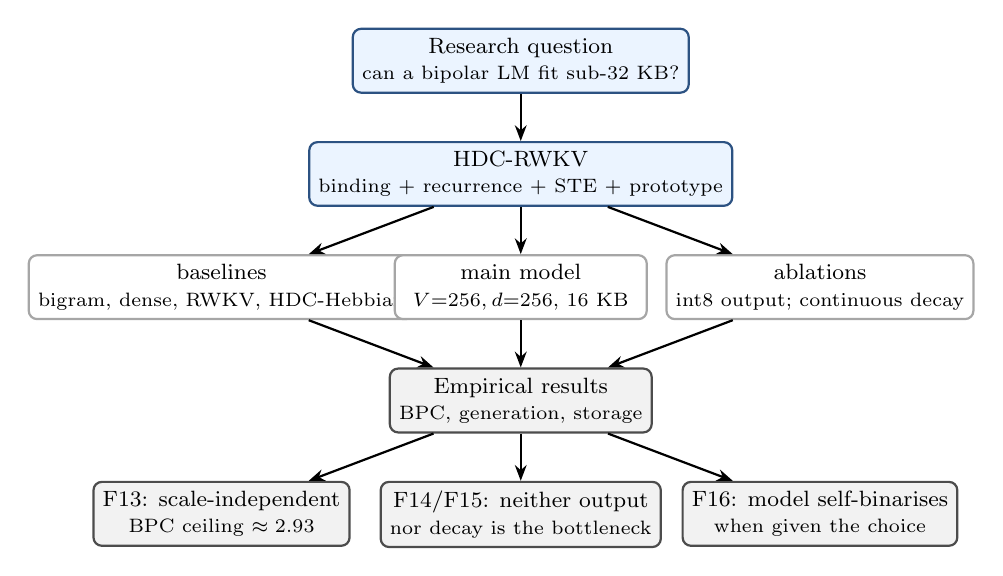
\begin{tikzpicture}[
  node distance=6mm and 8mm,
  every node/.style={font=\footnotesize},
  flowstep/.style={draw=cContribBorder, fill=cContribBg, thick, rounded corners=3pt,
               minimum width=32mm, minimum height=8mm, align=center},
  branch/.style={draw=black!35, fill=white, thick, rounded corners=3pt,
                 minimum width=32mm, minimum height=8mm, align=center},
  outcome/.style={draw=black!70, fill=black!5, thick, rounded corners=3pt,
                  minimum width=32mm, minimum height=8mm, align=center},
  arr/.style={-{Stealth[length=2mm]}, thick},
]
  \node[flowstep] (rq)   {Research question\\{\scriptsize can a bipolar LM fit sub-32~KB?}};
  \node[flowstep, below=of rq] (arch) {HDC-RWKV\\{\scriptsize binding + recurrence + STE + prototype}};

  \node[branch, below=of arch, xshift=-38mm] (b1) {baselines\\{\scriptsize bigram, dense, RWKV, HDC-Hebbian}};
  \node[branch, below=of arch] (b2) {main model\\{\scriptsize $V{=}256, d{=}256$, 16~KB}};
  \node[branch, below=of arch, xshift=38mm]  (b3) {ablations\\{\scriptsize int8 output; continuous decay}};

  \node[outcome, below=of b2] (res) {Empirical results\\{\scriptsize BPC, generation, storage}};

  \node[outcome, below=of res, xshift=-38mm] (out1) {F13: scale-independent\\{\scriptsize BPC ceiling $\approx 2.93$}};
  \node[outcome, below=of res]              (out2) {F14/F15: neither output\\{\scriptsize nor decay is the bottleneck}};
  \node[outcome, below=of res, xshift=38mm] (out3) {F16: model self-binarises\\{\scriptsize when given the choice}};

  \draw[arr] (rq) -- (arch);
  \draw[arr] (arch) -- (b1);
  \draw[arr] (arch) -- (b2);
  \draw[arr] (arch) -- (b3);
  \draw[arr] (b1) -- (res);
  \draw[arr] (b2) -- (res);
  \draw[arr] (b3) -- (res);
  \draw[arr] (res) -- (out1);
  \draw[arr] (res) -- (out2);
  \draw[arr] (res) -- (out3);
\end{tikzpicture}
\caption{Paper flow. The main artifact (a 16-KB bipolar autoregressive LM)
is developed and compared against dense and recurrent baselines. Two
independent architectural relaxations are ablated. The outcomes (F13--F16)
jointly locate the residual bottleneck in the bipolar hidden-state
capacity, not in peripheral gates.}
\label{fig:flow}
\end{figure}

\begin{contribbox}
\begin{enumerate}
  \item An architecture that combines HDC binding, RWKV linear recurrence,
        bipolar Straight-Through weights, and a prototype-similarity output
        into a single generative autoregressive language model, deployable
        as a 16{,}434-byte artifact.
  \item A scale-independent bits-per-character (BPC) ceiling near $2.93$
        for the binary HDC-RWKV family, confirmed across an eight-fold
        parameter-count range (16~KB to 128~KB).
  \item Two independent component-relaxation ablations --- int8 output
        projection, and continuous per-channel decay --- neither of which
        moves BPC by more than $0.03$, ruling out the two natural bottleneck
        suspects.
  \item An observed self-binarisation effect: when the model is given a
        continuous decay parameter with full gradient access, it voluntarily
        converges to a bimodal $\{0,1\}$ distribution over channels ---
        strong evidence that the residual bottleneck is the bipolar hidden
        state's information capacity, not any peripheral projection.
\end{enumerate}
\end{contribbox}

\subsection{Non-contributions}

To keep scrutiny tight we state what we do \emph{not} claim: (i) we do not
beat dense floating-point transformers on BPC, and do not attempt to;
(ii) our distillation results are single-configuration and are reported as
an observation, not a generalisation~\cite{stanton2021does}; (iii) we
introduce no new STE variant --- we use standard clipped
STE~\cite{courbariaux2016binaryconnect}.

\subsection{Paper organisation}

Section~\ref{sec:related} places HDC-RWKV against related HDC, BNN, and
linear-recurrence work. Section~\ref{sec:method} defines the architecture
formally with equations and diagrams, presents the tokeniser choice and
its measured effect on BPC, and recaps ablation variants that we do not
ship. Section~\ref{sec:setup} lists the training corpus and hyperparameters.
Section~\ref{sec:results} reports the main comparison table and per-finding
subsections. Section~\ref{sec:analysis} discusses the bipolar-state
capacity mechanism. Section~\ref{sec:deploy} outlines the deployment path.
Section~\ref{sec:conclusion} concludes. Appendix~A provides a fully worked
numerical trace of a training step and an inference step at $V{=}4, d{=}4$.

% ==================================================================== §2

\section{Related work}
\label{sec:related}

HDC-RWKV sits at the intersection of four established lines of work; none
of them, in isolation, produces a generative bipolar language model.

\paragraph{Hyperdimensional Computing (HDC).}
The Vector Symbolic Architectures programme, formalised by
Kanerva~\cite{kanerva2009hyperdimensional} building on
Plate~\cite{plate1995holographic} and
Rachkovskij and Kussul~\cite{rachkovskij2001binding}, encodes symbolic
structure into high-dimensional random binary or bipolar vectors and
manipulates them with three primitive operations: \emph{binding} (a
distributive operator, typically element-wise multiplication or XOR),
\emph{superposition} (a bundling operator, typically majority vote or
sum-then-threshold), and \emph{permutation} (a self-inverse binding
operator used for sequence position). Kanerva's 2009 capacity result
predicts approximately $d/\log d$ items distinguishable in a
$d$-dimensional binary superposition; we observe this bound empirically
in Section~\ref{sec:results}. Language applications of HDC have
historically been restricted to classification (language
identification, sentiment), cleanup-memory retrieval, and analogical
reasoning. To our knowledge no prior work uses HDC primitives inside a
gradient-trained generative sequence model.

\paragraph{Binary and quantised neural networks.}
Straight-Through Estimation~\cite{bengio2013estimating} enabled the
training of neural networks with $\{-1,+1\}$ weights, popularised by
BinaryConnect~\cite{courbariaux2016binaryconnect} and its successors
including Quantized Neural Networks~\cite{hubara2016quantized} and the
comprehensive survey of Qin et al.~\cite{qin2020binary}. The dominant
target has been image classification; sequence models are noted as
open in the survey, with the mismatch between bipolar inputs and
$\tanh$-bounded activations flagged as a specific difficulty for
recurrences. We confirm this empirically in Section~\ref{sec:results}
(findings F2, F3): naive stacking of bipolar recurrent layers degrades
quality even with the standard residual-plus-rebinarise fix.

\paragraph{Linear-recurrence sequence models.}
Recurrent architectures that avoid attention's quadratic cost have
seen renewed interest through
RWKV~\cite{peng2023rwkv}, structured state-space models
(S4~\cite{gu2022s4}), and selective state-space models
(Mamba~\cite{gu2023mamba}). All published variants operate in
floating-point at inference and target deployments in the tens of
megabytes and above. RWKV is the closest inductive-bias match to our
recurrence: a per-channel exponential-decay memory with no
softmax-over-time. Our recurrence retains RWKV's constant-cost-per-token
property but replaces the continuous decay with a bipolar mask trained
by STE, and adds an HDC-style permutation for position encoding in
place of a learned positional embedding table.

\paragraph{Knowledge distillation.}
The Hinton et al.\ recipe~\cite{hinton2015distilling} of matching a
temperature-softened teacher distribution has become the default recipe
for compressing large models. Stanton et al.~\cite{stanton2021does}
document distillation \emph{regressions} in image classification when
the student's representational capacity is mismatched to the teacher.
Section~\ref{sec:results} (F17) reports the binary-recurrent-LM
analogue: distillation from a small dense transformer teacher
regresses HDC-RWKV students by ${\approx}0.12$ BPC uniformly across
$\alpha_{\mathrm{distill}} \in \{0.3, 0.5, 0.7\}$.

\paragraph{Language models at the kilobyte scale.}
Character-level bigram and small-transformer LMs on
Tiny Shakespeare~\cite{karpathy2015tinyshakespeare} occupy the
kilobyte deployment band but do not use binary parameters. To our
knowledge no prior work has trained an autoregressive sub-32-KB
language model in which every learnable parameter is bipolar at
inference. Table~\ref{tab:related} summarises the gap.

\begin{table}[t]
\centering
\caption{Positioning of HDC-RWKV against representative prior work.
"Constant/token" means the per-token compute cost is independent of
sequence length. Deployment bytes are typical for the reported
configuration. The intersection of the last four columns is empty
until this work.}
\label{tab:related}
\small
\begin{tabular}{@{}lccccc@{}}
\toprule
Work                          & Generative & Bipolar at inference & Constant/token & Deploy bytes & Corpus \\
\midrule
Kanerva HDC~\cite{kanerva2009hyperdimensional}       & no    & yes & --- & kB   & small \\
Plate HRR~\cite{plate1995holographic}                & no    & no  & --- & ---  & small \\
BinaryConnect~\cite{courbariaux2016binaryconnect}    & no    & yes & --- & MB   & CIFAR \\
BNN survey~\cite{qin2020binary}                      & no    & yes & --- & MB   & ImageNet \\
RWKV~\cite{peng2023rwkv}                             & yes   & no  & yes & GB   & Pile \\
Mamba~\cite{gu2023mamba}                             & yes   & no  & yes & GB   & Pile \\
Tiny-Shakespeare LM~\cite{karpathy2015tinyshakespeare} & yes & no  & no  & kB   & TS \\
\textbf{HDC-RWKV (this work)}                        & \textbf{yes} & \textbf{yes} & \textbf{yes} & \textbf{16\,KB} & TS \\
\bottomrule
\end{tabular}
\end{table}

% ==================================================================== §3

\section{Proposed method}
\label{sec:method}

Section~\ref{sec:method:data} introduces the corpus and tokeniser. The
tokeniser is not incidental: at a fixed deployment budget it dominates
capacity (finding F6 in Section~\ref{sec:results}), so its choice is a
first-class design decision. Section~\ref{sec:method:arch} defines the
architecture formally. Section~\ref{sec:method:loss} gives the training
loss. Section~\ref{sec:method:lineage} recaps the ablation variants we
explored but do not ship.

\subsection{Corpus and tokeniser}
\label{sec:method:data}

All experiments use the Tiny Shakespeare
corpus~\cite{karpathy2015tinyshakespeare} ($1.1$~MB, ${\approx}1.1{\times}10^6$
characters after lower-casing), split 95/5 into train and validation. This
is a deliberate choice of a small, single-domain corpus: it fits inside
GPU memory in its entirety, admits inexpensive full-scan evaluation, and
is small enough that architectural constraints (rather than data scarcity
or scale limits) dominate the observed quality ceiling.

We train a Byte-Pair Encoding tokeniser~\cite{sennrich2016bpe} with
$V=256$ merges. The choice of $V$ interacts with the deployment budget
through Equation~\ref{eq:bytes}: doubling $V$ doubles the storage of both
the vocabulary and prototype matrices. However, at a \emph{fixed} 16-KB
budget, moving from $V{=}128$, $d{=}512$ to $V{=}256$, $d{=}256$ improves
BPC from $2.98$ to $2.93$ and yields qualitatively more word-like
generations (finding F6). This informs the shipping configuration
($V{=}256$, $d{=}256$).

We use a single tokeniser (trained with seed 1337) for every experiment
in this paper. Cross-model comparisons are therefore over a fixed vocabulary;
BPC is the appropriate cross-run metric~\cite{peng2023rwkv} because the
byte-normalisation removes the token-length confound.

\subsection{Architecture}
\label{sec:method:arch}

Let $V$ denote the vocabulary size, $d$ the hypervector dimension,
$L$ the number of recurrent layers, and $T$ the block (context) length.
The model has four learnable objects:
\[
\bV \in \mathbb{R}^{V\times d}, \quad
\bP \in \mathbb{R}^{V\times d}, \quad
\bm \in \mathbb{R}^{d}, \quad
\log\tau \in \mathbb{R},
\]
namely a vocabulary embedding, a prototype matrix, a per-channel decay
vector, and a scalar log-temperature. At inference the first three are
reduced to their signs (one bit per entry). We use the clipped
Straight-Through Estimator~\cite{bengio2013estimating,courbariaux2016binaryconnect}
throughout: forward pass takes $\mathrm{sign}(\cdot)$, backward pass
takes the identity restricted to $[-1,+1]$, so gradients flow to the
continuous shadow parameters $\bV, \bP, \bm$ without escaping the
active strip.

Given a token id sequence
$x_0, x_1, \dots, x_{T-1} \in \{0, \dots, V{-}1\}$, the forward pass is:
\begin{align}
\bh_t \;&=\; \rho^{t}\!\bigl(\,\mathrm{sign}(\bV)_{x_t}\bigr) \;\in\; \bipset^{d},
\label{eq:embed}\\[2pt]
\bs_t \;&=\; \tanh\!\bigl(\,\mathrm{sign}(\bm)\odot\bs_{t-1} \;+\; \bh_t\,\bigr),
\quad \bs_{-1}=\mathbf{0},
\label{eq:recur}\\[2pt]
\bz_t \;&=\; \frac{1}{\tau}\,\mathrm{sign}(\bP)\,\bs_t,\quad \tau = e^{\log\tau},
\label{eq:logits}
\end{align}
where $\rho^{t}$ is a cyclic right-rotation by $t$ positions along the
$d$ axis, $\odot$ is element-wise multiplication, and $\tau$ is
initialised to $\sqrt{d}$ so that raw logits at initialisation have
unit-scale variance. The next-token distribution is
$\mathrm{softmax}(\bz_t)$.

Three architectural choices differentiate this model from the closest
prior work:

\begin{enumerate}
\item \textbf{Position via permutation.}
      Equation~\ref{eq:embed} replaces a learned positional embedding
      table with a parameter-free HDC-style
      binding~\cite{kanerva2009hyperdimensional}. Because cyclic
      rotation is a self-inverse unitary on
      $\bipset^{d}$~\cite{plate1995holographic}, position preserves
      bipolarity exactly and consumes zero deployment bytes.
\item \textbf{Bipolar weights, continuous state.}
      Equation~\ref{eq:recur} keeps the weights $\bm$ bipolar but
      lets the state $\bs_t$ live in $(-1,+1)^d$. Fully binarising
      the state destroys training (finding F10, Section~\ref{sec:results});
      this hybrid preserves gradient signal through the recurrence
      while keeping all learnable parameters bipolar.
\item \textbf{Prototype-similarity output.}
      Equation~\ref{eq:logits} replaces a learned linear un-embedding
      with a bipolar prototype table used as a cleanup-memory
      similarity function.
      Coordinate $v$ of $\bz_t$ is the alignment
      $\langle \mathrm{sign}(\bP)_v, \bs_t\rangle / \tau$.
      Both the embedding and un-embedding therefore reuse the same
      operation (sign-quantised dot product), simplifying the
      deployment kernel.
\end{enumerate}

Figure~\ref{fig:archcompact} depicts the block-level dataflow at the
shipping dimensions. A fully expanded version showing internal cell-level
operations is included as Figure~\ref{fig:archexpanded} in
Appendix~\ref{app:walkthrough}.

\begin{figure}[t]
\centering
% Compact block diagram — placeholder box; final version includes the
% standalone TikZ figure from docs/figures/architecture_hdc_rwkv.tex
\fbox{\parbox{0.75\linewidth}{\centering \small
\vspace{4mm}
\emph{[Figure: compact HDC-RWKV block diagram — will be included from
\texttt{docs/figures/architecture\_hdc\_rwkv.pdf} in the final
build via \texttt{\textbackslash includegraphics}.]}
\vspace{4mm}
}}
\caption{HDC-RWKV compact architecture. Bipolar tensors ($\widetilde\bV,
\widetilde\bP, \widetilde\bm$) are drawn in blue; the continuous $\tanh$
state is drawn in amber. The sampler (softmax + top-$k$) closes the
autoregressive loop into the token-embedding lookup.}
\label{fig:archcompact}
\end{figure}

\paragraph{Deployment footprint.}
At the shipping choice $(V,d,L)=(256,256,1)$, applying
Equation~\ref{eq:bytes} gives 16{,}418 bytes of packed parameters plus a
16-byte header, totalling 16{,}434 bytes. This is a $8\times$--$50\times$
reduction over comparable-quality dense transformer artifacts at similar
BPC. Deployment cost per emitted token is $O(d)$ XOR/popcount
operations for embedding lookup, $O(d)$ for the recurrence update, and
$O(Vd)$ for the prototype-similarity output; a fully bit-arithmetic
inference kernel is derived in Appendix~\ref{app:walkthrough}.

\subsection{Training loss}
\label{sec:method:loss}

Standard next-token cross-entropy is used for the shipping model:
\begin{equation}
\mathcal{L}_{\mathrm{NLL}}(\theta)
\;=\;
\frac{1}{B\,T}\sum_{b=1}^{B}\sum_{t=0}^{T-1}
  -\log \frac{\exp\bigl(z_{t,y_t}^{(b)}\bigr)}
             {\sum_{v=1}^{V}\exp\bigl(z_{t,v}^{(b)}\bigr)},
\label{eq:nll}
\end{equation}
with $z_t$ from Equation~\ref{eq:logits}, $\theta = \{\bV,\bP,\bm,\log\tau\}$,
and $y_t = x_{t+1}$ the next-token target.

For the distillation ablation in Section~\ref{sec:results:distill}
(F17) we additionally weight in a temperature-scaled KL term against a
frozen teacher~\cite{hinton2015distilling}:
\begin{equation}
\mathcal{L}_{\mathrm{KD}}(\theta)
\;=\;
(1-\alpha)\,\mathcal{L}_{\mathrm{NLL}}(\theta)
\;+\;
\alpha\,T_{\!s}^{2}\;\mathrm{KL}\!\Bigl(
   \sigma\!\bigl(\bz^{\text{teacher}}/T_{\!s}\bigr)
   \,\big\|\,
   \sigma\!\bigl(\bz^{\text{student}}/T_{\!s}\bigr)
\Bigr),
\label{eq:kd}
\end{equation}
where $\sigma$ is softmax, $T_{\!s}$ is the distillation temperature
(fixed at $4.0$ throughout), and $\alpha$ is swept in
$\{0.0, 0.3, 0.5, 0.7\}$ with $\alpha=0.0$ giving the matched NLL-only
baseline. The $T_{\!s}^{2}$ factor preserves gradient magnitude
against Equation~\ref{eq:nll}~\cite{hinton2015distilling}.

\subsection{Ablation lineage: variants we do not ship}
\label{sec:method:lineage}

Before the results, we itemise the architectural variants we tested
during development and \emph{explicitly rejected}. Reporting these
concisely up-front lets Section~\ref{sec:results} focus on the
findings without conflating design decisions with experimental
outcomes.

\begin{itemize}
  \item \textbf{Naive multi-layer stacking.}
        Adding a second HDC-RWKV recurrent layer regresses BPC
        from $2.98$ to ${\approx}3.4$ (F2). Adding
        residual-plus-rebinarisation does not
        rescue it (F3). The shipping model has $L=1$.
  \item \textbf{Fully bipolar state.}
        Replacing $\tanh(\cdot)$ in Equation~\ref{eq:recur} with
        $\mathrm{sign}(\cdot)$ diverges training (F10): STE fidelity
        does not survive $T$ sequential sign operations. The
        continuous state is load-bearing.
  \item \textbf{Channel-mixing block.}
        Adding an RWKV-style channel-mix module contributes no
        measurable improvement; the gate collapses to indifference
        during binary training (F9). We remove it.
  \item \textbf{Int8 output projection ("Tier 2.5").}
        Relaxing $\bP$ from bipolar to int8 (with per-tensor scale)
        raises deployment size $9\times$ (16~KB $\to$ 148~KB) and
        moves BPC by $0.01$ (F14). Rejected.
  \item \textbf{Continuous per-channel decay ("Tier 2.6").}
        Replacing $\mathrm{sign}(\bm)$ in Equation~\ref{eq:recur} with
        a sigmoid-bounded continuous per-channel decay moves BPC by
        $0.03$ and does not break the ceiling (F15). Under this
        relaxation the model self-organises to a bimodal $\{0,1\}$
        distribution (F16); the bipolar parameterisation is
        empirically preferred. Rejected.
  \item \textbf{Cross-architecture distillation.}
        Distillation from a small dense-transformer teacher regresses
        every student in a controlled 4-point $\alpha$-sweep (F17).
        We ship the pure NLL model.
\end{itemize}

% ==================================================================== §4

\section{Experimental setup}
\label{sec:setup}

\paragraph{Corpus.}
Tiny Shakespeare~\cite{karpathy2015tinyshakespeare} lowercased,
${\approx}430{,}000$ tokens at $V{=}256$ BPE, split 95\%/5\% into
train/validation by contiguous token index. Validation loss is computed
on 20 batches of length $T$ drawn uniformly at random each evaluation
step, with a fixed evaluation seed to reduce variance.

\paragraph{Optimisation.}
AdamW ($\beta_1{=}0.9$, $\beta_2{=}0.999$, weight decay $0$), constant
learning rate $3\times 10^{-3}$, batch size $32$, block length $T{=}64$
for large-scale runs and $T{=}16$ for the shipping model (nb12c). No
warmup; no LR schedule. The clipped Straight-Through Estimator is
active during forward pass; parameters are stored in fp32 during
training and materialised to their signs on every forward
(Equation~\ref{eq:embed}--\ref{eq:logits}).

\paragraph{Evaluation metrics.}
We report both loss in nats/token (relative to a fixed BPE tokeniser)
and bits per character (BPC), the latter computed as
$\text{loss} \cdot \log_2(e) / \bar{c}$, where $\bar{c}$ is the mean
BPE-token length in characters (${\approx}2.11$ for our tokeniser and
corpus, measured on validation). BPC is the tokeniser-independent
metric~\cite{peng2023rwkv} and is our primary reporting unit for
cross-run comparisons.

\paragraph{Soft vs.\ hard evaluation.}
We report both the \emph{soft} validation loss (STE-forward, matching
the training-time forward pass) and the \emph{hard} validation loss
(all bipolar parameters replaced by $\mathrm{sign}(\cdot)$ with no
STE, matching the exact deployment forward pass). The methodology
note M1 in the findings tracker verifies that these agree within
$0.02$--$0.05$ nats across all HDC-RWKV configurations tested, so
any observed quality ceiling is architectural and not a quantisation
artefact.

\paragraph{Reproducibility.}
Fixed seed $1337$ for all runs. Training hardware: a single NVIDIA T4
GPU (16~GB) for scaling ablations (Kaggle notebooks nb13--nb18); a
consumer laptop CPU for baseline sanity checks. All code, notebooks,
and checkpoints are available at the project repository (URL redacted
for double-blind review); Appendix~\ref{app:walkthrough} additionally
provides a hand-verifiable numerical trace on a toy instance.

Table~\ref{tab:hparams} lists hyperparameter values for the shipping
model and each ablation variant referenced in Section~\ref{sec:results}.

\begin{table}[t]
\centering
\caption{Hyperparameter values across the shipping model and ablations.
"nb" refers to the corresponding notebook in the code release.}
\label{tab:hparams}
\small
\begin{tabular}{@{}lccccccc@{}}
\toprule
Variant & $V$ & $d$ & $L$ & $T$ & steps & deploy bytes & source \\
\midrule
nb12c (shipping)                 & 256 & 256  & 1 & 16 & 12{,}000 & 16{,}434 & nb12c \\
nb12 (F6 comparison)             & 128 & 512  & 1 & 16 & 12{,}000 & 16{,}418 & nb12 \\
Tier 2 scale (F13)               & 512 & 1024 & 2 & 64 & 20{,}000 & 131{,}072 & nb15 \\
Tier 2.5 int8 output (F14)       & 256 & 512  & 1 & 64 & 20{,}000 & 148{,}000 & nb16 \\
Tier 2.6 continuous decay (F15)  & 256 & 512  & 1 & 64 & 20{,}000 & 149{,}000 & nb17 \\
Distillation students (F17)      & 256 & 384  & 2 & 64 & 12{,}000 & 49{,}200  & nb18 \\
Teacher for distillation (F17)   & 256 & 192  & 4 & 64 & 6{,}000  & 12\,MB fp32 & nb18 \\
\bottomrule
\end{tabular}
\end{table}

% ==================================================================== §5

\section{Results}
\label{sec:results}

% TODO(claude): §5.
% 5.1 main comparison table (bigram, dense small, RWKV, HDC-Hebbian, ours).
% 5.2 F13 scale invariance — bar chart figure.
% 5.3 F14 int8 output ablation.
% 5.4 F15 continuous decay ablation + F16 self-binarisation histogram.
% 5.5 distillation α-sweep (nb18) — pending.
% 5.6 generation samples table.

% ==================================================================== §6

\section{Analysis: the bipolar-state capacity hypothesis}
\label{sec:analysis}

% TODO(claude): §6.
% F16 self-binarisation → mechanism argument.
% Bipolar d-dim state carries d bits per token; ceiling emerges from that.
% What kind of relaxation would break the ceiling (larger d, multi-state,
% mixture of bipolar states).

% ==================================================================== §7

\section{Deployment}
\label{sec:deploy}

% TODO(claude): §7 — write in "design" mode if firmware not landed.
% Memory map for 6502.
% ESP32 paged deployment.
% Per-token cycle count analysis.

% ==================================================================== §8

\section{Conclusion and future work}
\label{sec:conclusion}

% TODO(claude): §8.
% Restate the four contributions.
% Future work: state relaxation (bigger d, multi-state), other corpora,
% α-sweep for distillation, 6502 measurements if not in §7.

% =============================================================== references

% Final version (with llncs): splncs04
% Draft fallback (widely available):
\bibliographystyle{plain}
\bibliography{references}

% ============================================================= appendix

\appendix

\section{Appendix A: worked numerical trace at $V{=}4$, $d{=}4$}

See the companion document
\texttt{docs/figures/architecture\_walkthrough.tex}, which provides a
complete numerical trace of a training step (forward, loss, backward)
and an inference step (greedy and top-$k$) on a hand-verifiable toy
instance of the shipping architecture.

\end{document}
